\section{(Binary) Integer Linear Programming}

\subsection{Review of Linear Programming}
\label{subsec:review-of-linear-programming}

Recall that linear programs are a class of problems that have been well studied and can be solved quickly (in terms of asymptotics, this means they can be solved in polynomial time).

\begin{defn}[Linear program]
\label{defn:linear-program}
    Given $A \in \R^{m\times n}$, $b \in \R^m$, and $c \in \R^n$, a \textit{linear program} can be written in either standard form or canonical (also called symmetric) form as follows:
    \begin{multicols}{2}
        \noindent
        \begin{equation*}
        \begin{array}{lllr@{}l@{}l@{}}
        \text{standard form} 
            & (LP)  & \min  & c^T x &           \\
            &       & \st   & Ax    & {}= b     \\
            &       &       &  x    & {}\ge \Vec{0}
        \end{array}
        \end{equation*}
    
        \noindent
        \begin{equation*}
        \begin{array}{lllr@{}l@{}l@{}}
        \text{canonical form} 
            & (LP)  & \min  & c^T x &           \\
            &       & \st   & Ax    & {}\ge b   \\
            &       &       &  x    & {}\ge \Vec{0}.
        \end{array}
        \end{equation*}
    \end{multicols}
\end{defn}

In optimization, a given problem has a dual that is related to its primal form. In linear programming, the duality gap is 0 if and only if the optimal solution is feasible for both problems, which is helpful if one is easier to solve than the other.

\begin{defn}[Dual program]
    \label{defn:dual-program}
    Given $A \in \R^{m \times n}$, $b \in \R^m$, and $c \in \R^n$, a \textit{dual program} can be written in either standard form or canonical (also called symmetric) form as follows:
    \begin{multicols}{2}
        \noindent
        \begin{equation*}
        \begin{array}{lllr@{}c@{}}
        \text{standard form} 
            & (DP)  & \max  & b^T y &           \\
            &       & \st   & A^T y & {}\le c   \\
        \end{array}
        \end{equation*}
        
        \noindent
        \begin{equation*}
        \begin{array}{lllr@{}c@{}}
        \text{canonical form} 
            & (DP)  & \max  & b^T y &           \\
            &       & \st   & A^T y & {}\le c   \\
            &       &       &  y    & {}\ge \Vec{0}.
        \end{array}
        \end{equation*}
        \end{multicols}
\end{defn}

The notation used above will also be used throughout unless otherwise specified. Additionally, $ofv_P$ will denote the objective function value for a particular problem $(P)$ and $oofv_P$ will denote the optimal objective function value for a particular problem $(P)$. The subscript will be dropped when the problem of interest is clear.

We recall some immediate results that relate a linear program $(LP)$ to its dual program $(DP)$.

\begin{thm}[Weak duality for LPs]
    \label{thm:weak-duality-LP}
    If $x$ is feasible in $(LP)$ and $y$ is feasible in $(DP)$, then $ofv_{DP}(y) \le ofv_{LP}(x)$.
\end{thm}

\begin{thm}[Supervisor principle for LPs]
    \label{thm:supervisor-principle-LP}
    If $x$ is feasible in $(LP)$, $y$ is feasible in $(DP)$, and $ofv_{DP}(y) = ofv_{LP}(x)$, then $x$ is optimal in $(LP)$ and $y$ is optimal in $(DP)$.
\end{thm}

\begin{thm}[Strong duality for LPs]
    \label{thm:strong-duality-LP}
    If $(LP)$ is feasible and $(DP)$ is feasible, then there exists $x$ that is feasible in $(LP)$ and $y$ that is feasible in $(DP)$ such that $ofv_{DP}(y) = ofv_{LP}(x)$. Hence, $x$ is optimal in $(LP)$ and $y$ is optimal in $(DP)$.
\end{thm}


\subsection{Introduction of (Binary) Integer Linear Programs}
\label{subsec:introduction-of-ilps}

In general, solving integer linear/dual programs is NP-hard.

\begin{defn}[Integer linear/dual program]
    \label{def:integer-linear/dual-program}
    Given $A \in \R^{m \times n}$, $b \in \R^m$, and $c \in \R^n$, a (binary) integer linear program $(ILP)$ and its integer dual program $(IDP)$ in canonical form is written as
    \begin{multicols}{2}
        \noindent
        \begin{equation*}
        \begin{array}{llr@{}l@{}}
            (ILP)   & \min  & c^T x &                   \\
                    & \st   & Ax    & {}\ge b           \\
                    &       &  x    & {}\in \{0, 1\}^n
        \end{array}
        \end{equation*}
        
        \noindent
        \begin{equation*}
        \begin{array}{llr@{}l@{}}
            (IDP)   & \min  & b^T y &                   \\
                    & \st   & A^T y & {}\le c           \\
                    &       &  y    & {}\in \{0, 1\}^n.
        \end{array}
        \end{equation*}
    \end{multicols}
\end{defn}

\begin{rmk}
    \label{rmk:ilp-lp-inequalities}
    Since the feasible region for the $(ILP)$ is a subset of the feasible region for the $(LP)$ (with all else same), then $oofv_{LP} \le oofv_{ILP}$. By a similar argument, $oofv_{IDP} \le oofv_{DP}$. This gives the following relations, assuming existence of respective solutions,
    \[
        oofv_{IDP} \le oofv_{DP} = oofv_{LP} \le oofv_{ILP}.
    \]
\end{rmk}

The duality gap between a given $(ILP)$ and $(IDP)$ does not have strong guarantees like for linear programs. However, we do have the following results relating $(ILP)$ and $(IDP)$.

\begin{thm}[Weak duality for ILPs]
    \label{thm:weak-duality-ILP}
    If $x$ is feasible in $(ILP)$ and $y$ is feasible in $(IDP)$, then $ofv_{IDP}(y) \le ofv_{ILP}(x)$.
    
    \begin{proof}
        Since $x$ is feasible in the relaxation $(LP)$ of $(ILP)$ and $y$ is feasible in the relaxation $(DP)$ of $(IDP)$, by weak duality for LPs, $ofv_{IDP}(y) \le ofv_{DP}(y) \le ofv_{LP}(x) \le ofv_{ILP}(x)$.
    \end{proof}
\end{thm}

\begin{thm}[Supervisor principle for ILPs]
    \label{thm:supervisor-principle-ILP}
    If $x$ is feasible in $(ILP)$, $y$ is feasible in $(IDP)$, and $ofv_{IDP}(y) = ofv_{ILP}(x)$, then $x$ is optimal in $(ILP)$ and $y$ is optimal in $(IDP)$.
    
    \begin{proof}
        By weak duality for ILPs, $ofv_{ILP}$ is lower bounded by $ofv_{IDP}(y)$ for all $y$ feasible in $(IDP)$, so $x$ is optimal in $(ILP)$. By a similar argument, $y$ is optimal in $(IDP)$. Further, by a squeeze argument, $oofv_{IDP}(y) = oofv_{DP}(y) = oofv{LP}(x) = oofv_{ILP}(x)$.
    \end{proof}
\end{thm}

In general, we do not have an analogous strong duality relation between a given $(ILP)$ and $(IDP)$, so there could be a duality gap.

\begin{exm}
    Let $A = [2]$, $b = [1]$, and $c = [1]$. Then,
    \begin{multicols}{2}
        \noindent
        \begin{equation*}
        \begin{array}{llr@{}l@{}}
            (ILP)   & \min  &  x    &               \\
                    & \st   & 2x    & {}\ge 1       \\
                    &       &  x    & {}\in \{0, 1\}
        \end{array}
        \end{equation*}
        
        \noindent
        \begin{equation*}
        \begin{array}{llr@{}l@{}}
            (IDP)   & \max  &  y    &                   \\
                    & \st   & 2y    & {}\le 1           \\
                    &       &  y    & {}\in \{0, 1\}.
        \end{array}
        \end{equation*}
    \end{multicols}
    $oofv_{ILP} = 1$ since $x = 1$ is the only feasible solution for $(ILP)$. $oofv_{IDP} = 0$ since $y = 0$ is the only feasible solution for $(IDP)$. This gives a duality gap of 1. 
    
    However, the linear relaxations have optimal solutions $x = y = \frac12$ and $oofv_{LP} = oofv_{DP} = \frac12$, upholding strong duality for LPs.
\end{exm}

Since solving ILPs is NP-Hard in general, we can instead solve the LP relaxation in poly-time. If we obtain an optimal solution $x^*$ for the $LP$, we know the following about the ILP:
\begin{itemize}
    \item $oofv_{LP} \le oofv_{ILP}$
    \item if $x^*$ happens to be binary-valued, then $x^*$ is also optimal in ILP.
\end{itemize}

\begin{defn}[Dual problems]
    \label{def:dual-problems}
    Consider the problems
    \begin{multicols}{2}
        \noindent
        \begin{equation*}
        \begin{array}{lll@{}}
            (P)     & \min  &  f(x)     \\
                    & \st   &   x \in S \\
        \end{array}
        \end{equation*}
        
        \noindent
        \begin{equation*}
        \begin{array}{lll@{}}
            (Q)     & \min  &  g(y)     \\
                    & \st   &   y \in T. \\
        \end{array}
        \end{equation*}
    \end{multicols}
    If for all $x \in S$ and $y \in T$, $g(y) \le f(x)$, then we say $(P)$ and $(Q)$ are \textit{dual problems}.
\end{defn}


\subsection{Graph Theory}
\label{subsec:graph-theory}

\begin{defn}[Simple graph]
    \label{def:simple-graph}
    A \textit{simple graph} $G = (V, E)$ consists of 
    \begin{itemize}
        \item a set $V$ of vertices
        \item a set $E$ of 2-element subsets of $V$.
    \end{itemize}
    This definition does not allow for
    \begin{itemize}
        \item self-loops
            
\begin{tikzpicture}[node distance={15mm}, thick, main/.style = {draw, circle}, minimum size=1em]
                \node[main] (1) {};
                \draw (1) to [out=0,in=90,looseness=4] (1);
            \end{tikzpicture}
        \item parallel edges
            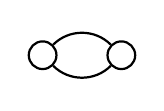
\begin{tikzpicture}[node distance={10mm}, thick, main/.style = {draw, circle}, minimum size=1em]
                \node[main] (1) {};
                \node[main] (2) [right of=1] {};
                \draw (1) to [out=45,in=135,looseness=1] (2);
                \draw (1) to [out=315,in=225,looseness=1] (2);
            \end{tikzpicture}
        \item directed edges
            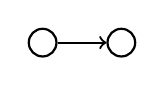
\begin{tikzpicture}[node distance={10mm}, thick, main/.style = {draw, circle}, minimum size=1em]
                \node[main] (1) {};
                \node[main] (2) [right of=1] {};
                \draw [->] (1) -- (2);
            \end{tikzpicture}
    \end{itemize}
\end{defn}

\begin{defn}[Matching]
    \label{def:matching}
    $F \sse E$ is a \textit{matching} if no 2 members of $F$ share endpoints. Note, $\emptyset$ is vacuously a matching. The \textit{matching number} $\alpha'(G)$ for a graph $G$ is
    \[
        \alpha'(G) \defeq \max_{F \sse E \text{ matching}} |F|.
    \]
    A \textit{perfect matching} is a matching that uses all vertices.
\end{defn}

\begin{defn}[Independent set]
    \label{def:independent-set}
    $S \sse V$ is an \textit{independent set} if no 2 members of $S$ are adjacent. Note, $\emptyset$ is vacuously an independent set. The \textit{independence number} $\alpha(G)$ for a graph $G$ is
    \[
        \alpha(G) \defeq \max_{S \sse V \text{ ind set}} |S|.
    \]
\end{defn}

\begin{defn}[Clique]
    \label{def:clique}
    $S \sse V$ is a \textit{clique} if every pair of vertices in $S$ are adjacent. Note, $\emptyset$ is vacuously a clique. The \textit{clique number} $\omega(G)$ for a graph $G$ is
    \[
        \omega(G) \defeq \max_{S \sse V \text{ clique}} |S|.
    \]
\end{defn}

\begin{exm}
    Consider the following example graph $\hat{G} = (V,E)$.
    \begin{center}
        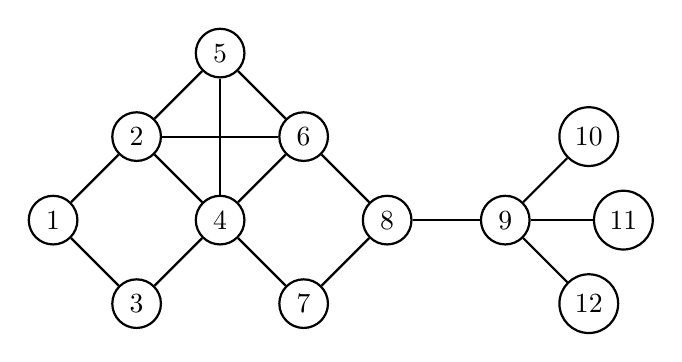
\begin{tikzpicture}[node distance={15mm}, thick, main/.style = {draw, circle}] 
            \node[main] (1) {$1$}; 
            \node[main] (2) [above right of=1] {$2$}; 
            \node[main] (3) [below right of=1] {$3$}; 
            \node[main] (4) [above right of=3] {$4$}; 
            \node[main] (5) [above right of=2] {$5$}; 
            \node[main] (6) [below right of=5] {$6$};
            \node[main] (7) [below right of=4] {$7$};
            \node[main] (8) [above right of=7] {$8$};
            \node[main] (9) [right of=8] {$9$};
            \node[main] (10) [above right of=9] {$10$};
            \node[main] (11) [right of=9] {$11$};
            \node[main] (12) [below right of=9] {$12$};
            \draw (1) -- (2);
            \draw (1) -- (3);
            \draw (2) -- (4);
            \draw (2) -- (5);
            \draw (2) -- (6);
            \draw (3) -- (4);
            \draw (4) -- (5);
            \draw (4) -- (6);
            \draw (4) -- (7);
            \draw (5) -- (6);
            \draw (6) -- (8);
            \draw (7) -- (8);
            \draw (8) -- (9);
            \draw (9) -- (10);
            \draw (9) -- (11);
            \draw (9) -- (12);
        \end{tikzpicture}
    \end{center}
    A matching is $\{(1,3), (4,5), (2,6), (7,8), (9,10)\}$. 
    An independent set is $\{1, 4, 8, 10, 11, 12\}$. 
    A clique is $\{2,4,6,8\}$. 
    Indeed these are all optimal and
    \begin{align*}
        \alpha'(\hat{G})    &= 5 \\
        \alpha(\hat{G})     &= 6 \\
        \omega(\hat{G})     &= 4.
    \end{align*}
    The independence number can be determined since one could partition $V$ into 6 cliques such that each clique is maximal.
\end{exm}

\begin{defn}[Vertex cover]
    \label{def:vertex-cover}
    $S \sse V$ is a \textit{vertex cover} if every edge of $E$ has an endpoint in $S$. The $\textit{vertex cover number}$ $\beta(G)$ for a graph $G$ is
    \[
        \beta(G) \defeq \min_{S \sse V \text{ vertex cover}} |S|.
    \]
\end{defn}

\begin{defn}[Edge cover]
    \label{def:edge-cover}
    $F \sse E$ is a \textit{edge cover} if every vertex of $V$ is an endpoint of an edge in $F$. The $\textit{edge cover number}$ $\beta'(G)$ for a graph $G$ is
    \[
        \beta'(G) \defeq \min_{F \sse E \text{ edge cover}} |F|.
    \]
\end{defn}

\begin{thm}[Weak duality for matchings and vertex covers]
    \label{thm:weak-duality-matchings-vertex-covers}
    For all graphs $G$, $\alpha'(G) \le \beta(G)$.
    
    \begin{proof}
        Let $F \sse E$ be a maximum matching and $S \sse V$ be a minimum vertex cover. For every edge of $F$, there exists an endpoint in $S$ by definition of a vertex cover. Let $M$ be the set of these vertices, which are all distinct by definition of a matching. Thus, $\alpha'(G) \equiv |F| = |M| \le |S| \equiv \beta(G)$.
    \end{proof}
\end{thm}

\begin{defn}[Bipartite graph]
    \label{def:bipartite-graph}
    A graph $G = (V, E)$ is \textit{bipartite} if $V$ can be partitioned into 2 independent sets $X$, $Y$, that is, every edge has an endpoint in $X$ and an endpoint in $Y$.
\end{defn}

\begin{thm}[K\"onig-Egervary]
    \label{thm:konig-egervary}
    If $G$ is bipartite, then $\alpha'(G) = \beta(G)$.
\end{thm}


\subsection{IPs with the Incidence Matrix}
\label{subsec:ips-with-incidence-matrix}

\begin{defn}[Incidence matrix]
    \label{def:incidence-matrix}
    Let $G = (V,E)$ be a simple graph, and say $V = \{v_1, v_2, \dots, v_n\}$ and $E = \{e_1, e_2, \dots, e_m\}$. The \textit{incidence matrix} $A_G$ of $G$ is the $m \times n$ binary matrix such that
    \[
        (A_G)_{ij} = \begin{cases}
                        1 & e_i \text{ has endpoint } v_j \\ 
                        0 & \text{else}
                     \end{cases}
        \quad \quad
        \forall i \in [m], j \in [n].
    \]
    We drop the subscript $G$ and use $A \equiv A_G$ when the context is clear.
\end{defn}

\begin{defn}[Indicator vector]
    To any set $S \sse V$, associate the \textit{indicator vector} $x_s \in \{0,1\}^n$ such that
    \[
        (x_S)_i \defeq \begin{cases}
                    1 & \text{if } v_i \in S \\
                    0 & \text{else}
                  \end{cases}
        \quad \quad
        \forall i \in [n].
    \]
    Similarly, to any set $F \sse E$, associate the indicator vector $y_F \in \{0,1\}^n$ such that
    \[
        (y_F)_i \defeq \begin{cases}
                    1 & \text{if } e_i \in F \\
                    0 & \text{else}
                  \end{cases}
        \quad \quad
        \forall i \in [m].
    \]
\end{defn}

\begin{exm}
    Consider the following graph $G = (V,E)$.
    \begin{center}
        \begin{tikzpicture}[node distance={15mm}, thick, main/.style = {draw, circle}] 
            \node[main] (1) {$v_1$};
            \node[main] (2) [right of=1] {$v_2$};
            \node[main] (3) [below right=1.6cm and 0.7cm of 5] {$v_3$};
            \node[main] (4) [right of=3] {$v_4$};
            \node[main] (5) [above right of=2] {$v_5$};
            \draw (1) -- (2) node[midway, below] {$e_1$};
            \draw (1) -- (5) node[midway, above left] {$e_4$};
            \draw (2) -- (3) node[midway, below] {$e_2$};
            \draw (2) -- (5) node[midway, left] {$e_5$};
            \draw (3) -- (4) node[midway, below] {$e_3$};
            \draw (3) -- (5) node[midway, right] {$e_6$};
            \draw (4) -- (5) node[midway, above right] {$e_7$};
        \end{tikzpicture}
    \end{center}
    The incidence matrix is
    \[
        A_G = \begin{bmatrix}
                1 & 1 & 0 & 0 & 0 \\
                0 & 1 & 1 & 0 & 0 \\
                0 & 0 & 1 & 1 & 0 \\
                1 & 0 & 0 & 0 & 1 \\
                0 & 1 & 0 & 0 & 1 \\
                0 & 0 & 1 & 0 & 1 \\
                0 & 0 & 0 & 0 & 1
              \end{bmatrix}.
    \]
    For a set $S = \{v_2, v_3, v_5\} \sse V$, the corresponding indicator vector is $x_S = \begin{bmatrix}0 & 1 & 1 & 0 & 1\end{bmatrix}^T$.
    For a set $F = \{e_3, e_4\} \sse E$, the corresponding indicator vector is $y_F = \begin{bmatrix}0 & 0 & 1 & 1 & 0 & 0 & 0\end{bmatrix}^T$.
\end{exm}

\begin{rmk}
    \label{rmk:incidence-matrix-inequality-iffs}
    Note the following equivalencies about vector inequalities with the incidence matrix:
    \begin{itemize}
        \item $\forall S \sse V$, $S$ is a vertex cover if and only if $A x_S \ge \one_m$
        \item $\forall F \sse E$, $F$ is a matching if and only if $A^T y_F \le \one_n$
        \item $\forall F \sse E$, $F$ is an edge cover if and only if $A^T y_F \ge \one_n$
        \item $\forall S \sse V$, $S$ is an independent set if and only if $Ax_S \le \one_m$
    \end{itemize}
\end{rmk}

From Remark \ref{rmk:incidence-matrix-inequality-iffs}, we can formulate two sets of dual IPs.

We begin with the min vertex cover and max matching problems. A dual relationship naturally arises -- given a matching $F$ for a graph $G$, which is a set of edges that do not share any endpoints, in order to form a vertex cover $S$ for $G$, we must include in $S$ at least one of the end of endpoints for each edge in $F$. Indeed, $S$ may require even more vertices to be a proper vertex cover, but we are guaranteed that $|S| \ge |F|$.

\begin{defn}[Min vertex cover problem]
    \label{def:min-vertex-cover-formulation}
    Given a graph $G=(V,E)$, we can formulate the \textit{min vertex cover problem} as:
        \begin{equation*}
        \begin{array}{llr@{}l@{}}
            (ILP)   & \min  &   \one_n^T x  &               \\
                    & \st   &       Ax      &{}\ge \one_m   \\
                    &       &       x       &{}\in \{0,1\}^n,
        \end{array}
        \end{equation*}
    where $A \equiv A_G$ and $x \equiv x_S$ for $S \sse V$. Indeed, any feasible solution is a vertex cover.
\end{defn}

\begin{defn}[Max matching problem]
    \label{def:max-matching-formulation}
    Given a graph $G=(V,E)$, we can formulate the \textit{max matching problem} as:
        \begin{equation*}
        \begin{array}{llr@{}l@{}}
            (IDP)   & \max  &   \one_m^T y  &               \\
                    & \st   &       A^T y   &{}\le \one_n   \\
                    &       &       y       &{}\in \{0,1\}^m,
        \end{array}
        \end{equation*}
    where $y \equiv y_F$ for $F \sse E$. Indeed, any feasible solution is a matching. Further, this problem is a dual of the min vertex cover problem.
\end{defn}

\begin{thm}[Weak duality]
    \label{thm:weak-duality-min-vtx-cover-max-matching}
    For all graph $G = (V,E)$, any matching $F$ and vertex cover $S$ satisfy $|F| \le |S|$.
\end{thm}

A second set of dual problems is the min edge cover and max independent set problems. Given an independent set $S$ for graph $G$, which is a set of vertices in which none of its vertices are adjacent, we need at least $|S|$ edges to cover $V$ since we will need at least $|S|$ edges to cover the vertices included in $S$.

\begin{defn}[Min edge cover problem]
    \label{def:min-edge-cover-formulation}
    Given a graph $G=(V,E)$, we can formulate the \textit{min edge cover problem} as:
        \begin{equation*}
        \begin{array}{llr@{}l@{}}
            (ILP)   & \min  &   \one_n^T y  &               \\
                    & \st   &       A^T y   &{}\ge \one_m   \\
                    &       &       y       &{}\in \{0,1\}^m,
        \end{array}
        \end{equation*}
    where $y \equiv y_F$ for $F \sse E$. Indeed, any feasible solution is a min edge cover.
\end{defn}

\begin{defn}[Max independent set problem]
    \label{def:max-ind-set-formulation}
    Given a graph $G=(V,E)$, we can formulate the \textit{max matching problem} as:
        \begin{equation*}
        \begin{array}{llr@{}l@{}}
            (IDP)   & \max  &   \one_n^T x  &               \\
                    & \st   &       Ax      &{}\le \one_m   \\
                    &       &       x       &{}\in \{0,1\}^n,
        \end{array}
        \end{equation*}
    where $x \equiv x_S$ for $S \sse V$. Indeed, any feasible solution is an independent set. Further, this problem is a dual of the min edge cover problem.
\end{defn}

\begin{thm}[Weak duality]
    \label{thm:weak-duality-min-edge-cover-max-ind-set}
    For all graph $G = (V,E)$, any edge cover $F$ and independent set $S$ satisfy $|S| \le |F|$.
\end{thm}


\subsection{IPs with Graph Colorings}
\label{subsec:ips-with-graph-colorings}

\begin{defn}[Vertex Coloring]
    \label{def:vertex-coloring}
    For a graph $G = (V,E)$, a \textit{(proper) vertex coloring} of $G$ is an assignment $\theta: V \rightarrow \{1, 2, 3, \dots\}$ of a color to each vertex such that every pair of adjacent vertices, the two vertices have different colors. The \textit{chromatic number} $\chi(G)$ for a graph $G$ is defined as the fewest number of colors needed to properly color $G$.
\end{defn}

\begin{exm} 
    Consider the following graph $\hat{G}$.
    \begin{center}
        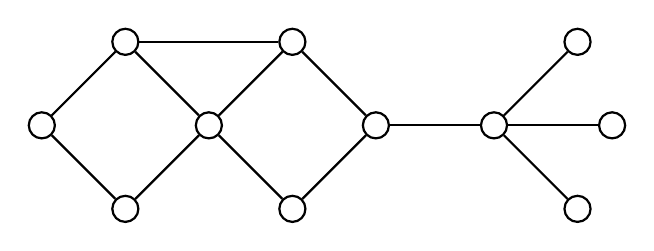
\begin{tikzpicture}[node distance={15mm}, thick, main/.style = {draw, circle}] 
            \node[main] (1) {}; 
            \node[main] (2) [above right of=1] {}; 
            \node[main] (3) [below right of=1] {}; 
            \node[main] (4) [above right of=3] {}; 
            \node[main] (5) [above right of=4] {};
            \node[main] (6) [below right of=4] {};
            \node[main] (7) [above right of=6] {};
            \node[main] (8) [right of=7] {};
            \node[main] (9) [above right of=8] {};
            \node[main] (10) [right of=8] {};
            \node[main] (11) [below right of=8] {};
            \draw (1) -- (2);
            \draw (1) -- (3);
            \draw (2) -- (4);
            \draw (2) -- (5);
            \draw (3) -- (4);
            \draw (4) -- (6);
            \draw (4) -- (5);
            \draw (5) -- (7);
            \draw (6) -- (7);
            \draw (7) -- (8);
            \draw (8) -- (9);
            \draw (8) -- (10);
            \draw (8) -- (11);
        \end{tikzpicture}
    \end{center}
    
    Observe that because there is a 3-clique, which requires $\chi(G) \ge 3$. The following is a vertex coloring showing that $\chi(G) = 3$.
    \begin{center}
        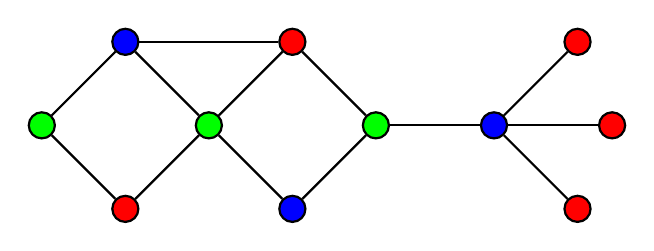
\begin{tikzpicture}[node distance={15mm}, thick, main/.style = {draw, circle}] 
            \node[main, fill=green] (1) {}; 
            \node[main, fill=blue] (2) [above right of=1] {}; 
            \node[main, fill=red] (3) [below right of=1] {}; 
            \node[main, fill=green] (4) [above right of=3] {}; 
            \node[main, fill=red] (5) [above right of=4] {};
            \node[main, fill=blue] (6) [below right of=4] {};
            \node[main, fill=green] (7) [above right of=6] {};
            \node[main, fill=blue] (8) [right of=7] {};
            \node[main, fill=red] (9) [above right of=8] {};
            \node[main, fill=red] (10) [right of=8] {};
            \node[main, fill=red] (11) [below right of=8] {};
            \draw (1) -- (2);
            \draw (1) -- (3);
            \draw (2) -- (4);
            \draw (2) -- (5);
            \draw (3) -- (4);
            \draw (4) -- (6);
            \draw (4) -- (5);
            \draw (5) -- (7);
            \draw (6) -- (7);
            \draw (7) -- (8);
            \draw (8) -- (9);
            \draw (8) -- (10);
            \draw (8) -- (11);
        \end{tikzpicture}
    \end{center}
\end{exm}

\begin{thm}[Weak duality]
    \label{thm:weak-duality-max-clique-min-coloring}
    For all graphs $G$, $\omega(G) \le \chi(G)$.
\end{thm}

Note that each color class (vertices with the same color) form an independent set. This gives the following observation.
\begin{obs}
    A vertex coloring is a partition of the vertices into independent sets. Thus, $\chi(G)$ can be thought of as the fewest number of independent sets in a partition of vertices of $G$ into independent sets.
\end{obs}

\begin{defn}
    For a graph $G = (V,E)$, where say $V=\{v_1, v_2, \dots, v_n\}$, let all possible independent sets be enumerated as $I_1, I_2, \dots, I_l$. Define the binary matrix $M \in \{0,1\}^{n\times l}$ such that
    \[
        M_{ij} \defeq \begin{cases}
                        1 & \text{if } v_i \in I_j \\
                        0 & \text{else}
                      \end{cases}
    \]
\end{defn}

\begin{exm}
    Consider the following graph
    \begin{center}
        \begin{tikzpicture}[node distance={15mm}, thick, main/.style = {draw, circle}] 
            \node[main] (1) {$v_1$};
            \node[main] (2) [right of=1] {$v_2$};
            \node[main] (3) [below right=0.625cm and 0.1cm of 5] {$v_3$};
            \node[main] (4) [right of=3] {$v_4$};
            \node[main] (5) [above right of=2] {$v_5$};
            \draw (1) -- (2);
            \draw (1) -- (5);
            \draw (2) -- (3);
            \draw (2) -- (5);
            \draw (3) -- (4);
            \draw (3) -- (5);
            \draw (4) -- (5);
        \end{tikzpicture}
    \end{center}
    The matrix $M$ for this graph is
    \[
        M = \left[
            \begin{array}{c:ccccc:ccc}
                0 & 1 & 0 & 0 & 0 & 0 & 1 & 1 & 0 \\ 
                0 & 0 & 1 & 0 & 0 & 0 & 0 & 0 & 1 \\ 
                0 & 0 & 0 & 1 & 0 & 0 & 1 & 0 & 0 \\
                0 & 0 & 0 & 0 & 1 & 0 & 0 & 1 & 1 \\
                0 & 0 & 0 & 0 & 0 & 1 & 0 & 0 & 0
            \end{array}
            \right].
    \]
    The dashed lines indicate different ``types" of independent sets of the graph.
    The first column is the empty independent set,
    the next five are trivial singleton independent sets, and
    the last three are non-trivial independent sets.
\end{exm}

\begin{defn}[Independent set covering]
    \label{def:ind-set-covering}
    An \textit{independent set covering} (aka a vertex coloring) is a collection $\Cal{I} \sse\{I_1, I_2, \dots, I_n\}$ of independent sets such that $\bigcup_{I_i \in \Cal{I}} I_i = V$. Further, for all $\Cal{I} \sse \{I_1, I_2, \dots, I_n\}$, define the indicator vector $x_{\Cal{I}} \in \{0,1\}^l$ such that
    \[
        (x_{\Cal{I}})_i \defeq \begin{cases}
                                1 & \text{if } I_i \in \Cal{I} \\
                                0 & \text{else}.
                               \end{cases}
    \]
\end{defn}

\begin{exm}
    Consider the same graph as the previous example.
    \begin{center}
        \begin{tikzpicture}[node distance={15mm}, thick, main/.style = {draw, circle}] 
            \node[main] (1) {$v_1$};
            \node[main] (2) [right of=1] {$v_2$};
            \node[main] (3) [below right=0.51cm and 0.1cm of 5] {$v_3$};
            \node[main] (4) [right of=3] {$v_4$};
            \node[main] (5) [above right=0.625cm and 0.1cm of 2] {$v_5$};
            \draw (1) -- (2);
            \draw (1) -- (5);
            \draw (2) -- (3);
            \draw (2) -- (5);
            \draw (3) -- (4);
            \draw (3) -- (5);
            \draw (4) -- (5);
        \end{tikzpicture}
    \end{center}
    
    Consider the following two indicator vectors
    \begin{multicols}{2}
        \noindent\[
            x_{\Cal{I}_1} = \begin{bmatrix} 
                                0 \\ 0 \\ 0 \\ 1 \\ 0 \\ 0 \\ 0 \\ 0 \\ 1
                            \end{bmatrix}
        \]
        \noindent\[ 
            x_{\Cal{I}_2} = \begin{bmatrix} 
                                0 \\ 0 \\ 0 \\ 0 \\ 0 \\ 1 \\ 1 \\ 0 \\ 1
                            \end{bmatrix}
        \]
    \end{multicols}
    Since $Mx_{\Cal{I}_1} \not\ge \one$, then there is at least one vertex not being covered by an independent set of $\Cal{I}_1$. In contrast, $Mx_{\Cal{I}_2} \ge \one$, so $\Cal{I}_2$ is an independent set covering, i.e. a proper vertex coloring.
\end{exm}

We formulate the min chromatic number and max clique problems, which are dual problems as suggested by Theorem \ref{thm:weak-duality-max-clique-min-coloring}.

\begin{defn}[Min chromatic number problem]
    \label{def:min-chromatic-number-formulation}
    Given a graph $G = (V,E)$, we can formulate the \textit{min chromatic number problem} as:
        \begin{equation*}
            \begin{array}{llr@{}l@{}}
                (ILP)   & \min  &   \one_l^T x  &               \\
                        & \st   &       Mx      &{}\ge \one_n   \\
                        &       &       x       &{}\in \{0,1\}^l
            \end{array}
        \end{equation*}
\end{defn}

\begin{defn}[Max clique problem]
    \label{def:max-clique-formulation}
    Given a graph $G = (V,E)$, we can formulate the \textit{max clique problem} as:
        \begin{equation*}
            \begin{array}{llr@{}l@{}}
                (IDP)   & \max  &   \one_n^T y  &               \\
                        & \st   &       M^T y   &{}\le \one_l   \\
                        &       &       y       &{}\in \{0,1\}^n,
            \end{array}
        \end{equation*}
    where $y$ is the indicator vector for a set $S$ of vertices. Note that $(M^T y)_i = |S \cap I_i|$. So if $|S \cap I_i| \le 1$ for all $i \in [l]$, then $S$ is a clique, otherwise if more than 1 vertex of $S$ was in an independent set, then those vertices are not adjacent, and $S$ therefore cannot be a clique. Conversely, if $S$ is not a clique, then it will an intersection with an independent set with size at least 2.
\end{defn}

\begin{exm}
    Observe the following graph that demonstrates a duality gap:
    \begin{center}
        \begin{tikzpicture}[node distance={15mm}, thick, main/.style = {draw, circle}]
            \node[draw, regular polygon,regular polygon sides=5,minimum size=2cm] (p) {};
                \foreach\x in {1,...,5}{
                    \node[main=\x, fill=white] (p\x) at (p.corner \x){};
                }
        \end{tikzpicture}
    \end{center}
    
    This graph has $\omega(G) = 2$, but $\chi(G) = 3$.
\end{exm}


\subsection{Magic Squares}
\label{subsec:magic-squares}

\begin{defn}
    \label{def:magic-square}
    An $n \times n$ \textit{magic square} is an $n \times n $ matrix $M$ such that all integers $1, 2, \dots, n^2$ are used once as entries and that all row and column sums are all equal.
\end{defn}

\begin{exm}
    The following is a $3\times3$ magic square:
    \[
        M = \begin{bmatrix}
                4 & 9 & 2 \\
                3 & 5 & 7 \\
                8 & 1 & 6
            \end{bmatrix}
    \]
    Observe that the row and column sums are all 15.
\end{exm}

\begin{obs}
    The row and column sum value $s$ for any arbitrary $n \times n$ magic square $M$ can be derived. Since the sum of all entries of $M$ must be $ns$, then 
    \begin{alignat*}{2}
        &                   & ns    &= 1 + 2 + \cdots + n^2  \\
        &                   &       &=\frac{n^2(n^2+1)}{2} \\
        & \Longrightarrow   & s     &= \frac{n(n^2+1)}{2}
    \end{alignat*}
\end{obs}

\begin{obs}
    There is no $2 \times 2$ magic square. If such a magic square existed, it would need to be symmetric for the row and column sums to be equal, but all entries must be distinct, therefore such a magic square would be a contradiction to the definition.
\end{obs}

\begin{defn}
    For all $i = 1, 2, \dots, n$ $j = 1,2,\dots,n$, and $k = 1,2,\dots, n^2$, define
    \[
        x_{ijk} = \begin{cases}
                    1 & \text{if } m_{ij} = k \\
                    0 & \text{else}
                  \end{cases}
    \]
    This tells us that the number of decision variables for a magic square problem is $n \cdot n \cdot n^2 = n^2$.
\end{defn}

\noindent We can encode the constraints for a magic square as follows:
\begin{itemize}
    \item Requiring only one integer entry for $m_{ij}$
    \[
        \forall i \in [n], j \in [n] \quad\quad \sum_{k=1}^{n^2} x_{ijk} = 1
    \]
    \item Requiring each $k \in [n^2]$ to appear exactly once in $M$
    \[
        \forall k \in [n^2] \quad\quad \sum_{i=1}^n\sum_{j=1}^n x_{ijk} = 1
    \]
    \item Requiring row sums to be $s$
    \[
        \forall i \in [n] \quad\quad \sum_{j=1}^n\sum_{k=1}^{n^2} kx_{ijk} = s
    \]
    \item Requiring column sums to be $s$
    \[
        \forall j \in [n] \quad\quad \sum_{i=1}^n\sum_{k=1}^{n^2} kx_{ijk} = s
    \]
\end{itemize}
This gives a total of $2n^2 + 2n$ constraints, and since there are $n^4$ variables, the magic square problem is underconstrained.

\noindent Formulating these constraints as part of an optimization problem, we have 
    \[
        Ax = b,
    \]
where $A \in \Z^{(2n^2+2n) \times n^4}$, $b \in \Z^{2n^2+2n}$, and $x \in \{0,1\}^{n^4}$. Note that the decision variables $x$ has been vectorized into a long vector, so $x_{ijk}$ corresponds to the index $(i-1) \cdot n \cdot n^2 + (j-1)\cdot n^2 + (k-1) + 1$ in the optimization problem formulation version of $x$.

The following is MATLAB code to naively implement the above constraints
\begin{lstlisting}
    % magicSquare.m
    %% one integer in each entry m_ij
    row = 0
    for i = 1:n
        for j = 1:n
            row = row + 1
            for k = 1:n^2
                A(row, (i-1)*n*n^2 + (j-1)*n^2 + (k-1) + 1) = 1
            end
            b(row) = 1
        end
    end
    
    %% all row sums are equal to s
    for i = 1:n
        row = row + 1
        for j = 1:n
            for k = 1:n^2
                A(row, (i-1)*n*n^2 + (j-1)*n^2 + (k-1) + 1) = k
            end
        end
        b(row) = s
    end
\end{lstlisting}

In the case where we are partially given a magic square with set entries, then we can partition our constraint as follows
\begin{alignat*}{2}
    &&Ax &= b \\
    &\Longrightarrow \quad & [\begin{array}{c|c} B & N\end{array}] \begin{bmatrix}
    x_B \\ x_N \end{bmatrix} &= b \\
    &\Longrightarrow \quad & Bx_B + Nx_N &= b \\
    &\Longrightarrow \quad & \underbrace{B}_{``\hat{A}"}x_B &= \underbrace{b-Nx_N}_{``\hat{b}"}
\end{alignat*}